% Provenance (never printed): sources/book2/BRIEFS.md, g11-12. Survey definitions; stocks and flows and the steady state;
% frictional, structural and cyclical unemployment; why wages do not clear the market; benefits and the evidence.
% Real numbers: figdata/grade-11/12-unemployment/ (Eurostat une_rt_a 2024; JST unemp 1870-2020, the US 2019 value from WDI;
% Brenland flows, invented). Ledger: Eurostat ILO definition, Shimer 2007/2012, Raff and Summers 1987, Card, Chetty and
% Weber 2007. No employment-protection estimate was read; none is cited. The diagram of a wage above the clearing level (see
% the minimum-wage diagram of the labour-market chapter) was not added. Photograph: a 1932 breadline (Commons, PD).
\chapter{Unemployment}\label{ch:g11:unemployment}

In 2024, 6.6\,\% of Germans aged 15 to 24 who were working or looking for work were unemployed. In Spain the figure was 26.5\,\%; in Sweden, 24.3\,\%. For all ages from
15 to 74, the rates were 3.5\,\% in Germany, 11.4\,\% in Spain and 8.4\,\% in Sweden. These are rich countries, open to each other's trade, in the same year; Germany's output was even
shrinking, by 0.5\,\%, while Spain's grew by 3.5\,\%. Their unemployment rates differ by a factor of three.
% figdata: eu_unemp (DE 6.6/3.5, ES 26.5/11.4, SE 24.3/8.4); growth_2024 (DEU -0.50, ESP 3.46, SWE 1.02)

Unemployment is not one thing. Some of it is the normal time it takes to find a job; some reflects a lasting mismatch between workers and jobs, or rules that keep
wages from adjusting; some rises and falls with recessions. This chapter defines the measures precisely, builds a model of the flows into and out of unemployment, and
reviews what the evidence says about the main causes and policies.

\begin{openingchart}{Unemployment rate, ages 15--24 and 15--74, fifteen European countries and the European Union, 2024, in per cent of the labour force of that
age.}{Eurostat, Labour Force Survey (une\_rt\_a)}
\begin{tikzpicture}
\begin{axis}[width=0.92\linewidth, height=5.6cm, ybar, /pgf/bar width=4.5pt, xtick={0,...,15}, xticklabels={DE, CZ, PL, NL, IE, AT, DK, BE, IT, PT, FI, FR, EL, SE,
  ES, EU}, enlarge x limits=0.04, ymin=0, ymax=30, ylabel={per cent}, legend style={at={(0.02,0.98)}, anchor=north west, font=\scriptsize, draw=none},
  legend columns=2, x tick label style={/tikz/font=\scriptsize}]
\addplot[fill=omThm!60, draw=omThm] table[x=x, y=youth] {figdata/grade-11/12-unemployment/out/eu_unemp.csv};
\addplot[fill=omDef!60, draw=omDef] table[x=x, y=total] {figdata/grade-11/12-unemployment/out/eu_unemp.csv};
\legend{ages 15--24, ages 15--74}
\end{axis}
\end{tikzpicture}
\end{openingchart}

\begin{recall}
From the grades 6--9 volume: the labour force, the unemployment rate and the participation rate, and the survey that measures them. From
\cref{ch:g11:labour-market}: the \omterm{def:g11:labour-market:minimum-wage}{minimum wage} and the two models of its effect. From the mathematics volumes: sequences defined by $u_{t+1} = a + b\,u_t$ and their limit
when $|b| < 1$.
\end{recall}

\section{Who counts as unemployed}\label{sec:g11:unemployment:definitions}

\begin{definition}[ILO unemployment]\label{def:g11:unemployment:ilo}
A person is unemployed in the sense of the International Labour Organization, \emph{ILO unemployment}\index{ILO unemployment}, if he or she is of working age, did no
paid work in the reference week, is available to start work soon, and has actively looked for work recently (or has found a job that starts soon).
\end{definition}

\begin{measure}[Who counts as unemployed]
% ledger: g11:ilo-unemployed
Eurostat applies the ILO guidelines this way: a person aged 15 to 74 who was not employed in the reference week, could start work within two weeks, and actively looked for
work during the four weeks ending with that week, or has found a job that starts within three months. Someone who
wants a job but has stopped looking is not unemployed but \emph{inactive}; so is someone who is looking but cannot start within two weeks.
\end{measure}

\begin{definition}[Employment rate and underemployment]\label{def:g11:unemployment:employment-rate}
The \emph{employment rate}\index{employment rate} is the number employed divided by the working-age population. \emph{Underemployment}\index{underemployment}%
\phantomsection\label{def:g11:unemployment:underemployment} is the situation of people who work part time but want, and are available for, more hours.
\end{definition}

The unemployment rate divides by the labour force, the \omterm{def:g11:unemployment:employment-rate}{employment rate} by the whole population. A fall in the unemployment rate can come from more people finding jobs
or from more people giving up the search; the \omterm{def:g11:unemployment:employment-rate}{employment rate} tells the two apart.

\section{Flows into and out of unemployment}\label{sec:g11:unemployment:flows}

\begin{definition}[Separation and job-finding rates]\label{def:g11:unemployment:separation-rate}
The \emph{separation rate}\index{separation rate} $s$ is the share of the employed who lose or leave their job in a period and become unemployed. The \emph{job-finding
rate}\index{job-finding rate}\phantomsection\label{def:g11:unemployment:job-finding-rate} $f$ is the share of the unemployed who find a job in a period.
\end{definition}

\begin{omfigure}
\begin{tikzpicture}[font=\small]
\node[draw, rounded corners, minimum width=3.2cm, minimum height=1.1cm, fill=omDef!12] (E) at (0,0) {employed $1 - u$};
\node[draw, rounded corners, minimum width=3.2cm, minimum height=1.1cm, fill=omThm!12] (U) at (6,0) {unemployed $u$};
\draw[->, thick] (E.north east) to[bend left=25] node[above, font=\scriptsize] {separations $s(1 - u)$} (U.north west);
\draw[->, thick] (U.south west) to[bend left=25] node[below, font=\scriptsize] {job findings $f u$} (E.south east);
\end{tikzpicture}

{\small The labour force as two boxes. Each period a share $s$ of the employed become unemployed and a share $f$ of the unemployed find work. Movements in and out of the
labour force are left aside.}
\end{omfigure}

As shares of a labour force of fixed size, the unemployment rate moves by inflows minus outflows:
\[ u_{t+1} = u_t + s(1 - u_t) - f u_t = s + (1 - s - f)\,u_t. \]

\begin{proposition}[The steady-state rate]\label{prop:g11:unemployment:steady}
If $s$ and $f$ are constant, with $0 < s + f < 2$, the unemployment rate converges to $u^* = s/(s + f)$, and the gap $u_t - u^*$ is multiplied by $1 - s - f$ each period.
\end{proposition}
\begin{proof}
$u^*$ is the fixed point: $u^* = s + (1 - s - f)u^*$ gives $u^*(s + f) = s$. Subtracting it from the recurrence, $u_{t+1} - u^* = (1 - s - f)(u_t - u^*)$, so
$u_t - u^* = (1 - s - f)^t (u_0 - u^*)$, which tends to 0 since $|1 - s - f| < 1$.
\end{proof}

With monthly rates of $s = 0.01$ and $f = 0.24$, the steady state is $0.01/0.25 = 4\,\%$, and a gap closes by a quarter each month. The model shows that the same rate can
come from few people losing jobs and staying out long, or from many losing jobs and finding new ones fast; the two call for different explanations.

\begin{model}{The stock--flow model of unemployment}
\assumes Constant separation and \omterm{def:g11:unemployment:separation-rate}{job-finding rates}; a labour force of fixed size.
\predicts Unemployment converges to $s/(s + f)$; a fall in the \omterm{def:g11:unemployment:separation-rate}{job-finding rate} raises it, a rise in the \omterm{def:g11:unemployment:separation-rate}{separation rate} too.
\tested In the United States since 1948, changes in the \omterm{def:g11:unemployment:separation-rate}{job-finding rate} account for about three-quarters of the swings in the unemployment rate and changes in the
  \omterm{def:g11:unemployment:separation-rate}{separation rate} for about a quarter (Shimer 2012).
\breaks The rates are not constant: both move with the business cycle, and the \omterm{def:g11:unemployment:separation-rate}{job-finding rate} falls the longer a person has been out of work.
\end{model}
% ledger: g11:shimer

The chart below applies the model to two groups of workers in Brenland, through a recession that lowers their \omterm{def:g11:unemployment:separation-rate}{job-finding rates} for a year; the weekend problem works
through its numbers.

\begin{omchart}{Brenland's unemployment rate by group and overall, month by month, through a twelve-month recession and the two years after (invented; the weekend
problem).}{invented data}
\begin{tikzpicture}
\begin{axis}[omtime, width=0.8\linewidth, height=5.0cm, xmin=0, xmax=36, ymin=0, ymax=17, xlabel={month}, ylabel={per cent}, xtick={0,6,...,36},
]
\addplot[omDef, thick] table[x=month, y=A] {figdata/grade-11/12-unemployment/out/bren_path.csv}
  node[pos=0.75, below, font=\scriptsize] {group A};
\addplot[omThm, thick] table[x=month, y=B] {figdata/grade-11/12-unemployment/out/bren_path.csv}
  node[pos=0.75, above, font=\scriptsize] {group B};
\addplot[black, thick, dashed] table[x=month, y=all] {figdata/grade-11/12-unemployment/out/bren_path.csv}
  node[pos=0.75, above, font=\scriptsize] {Brenland};
\end{axis}
\end{tikzpicture}
\end{omchart}
% figdata: bren_key (4, 10, 5.5; 6.25, 16.67; 5.97, 15.23, 8.29; 2.4, 3.1)

\begin{definition}[Long-term unemployment]\label{def:g11:unemployment:long-term}
\emph{Long-term unemployment}\index{long-term unemployment} is unemployment that has lasted a year or more.
\end{definition}

\section{Three kinds of unemployment}\label{sec:g11:unemployment:kinds}

\begin{definition}[Frictional, structural and cyclical unemployment]\label{def:g11:unemployment:frictional}
\emph{Frictional unemployment}\index{frictional unemployment} is the unemployment of people between jobs, which comes from the time it takes to match workers and jobs.
\emph{Structural unemployment}\index{structural unemployment}\phantomsection\label{def:g11:unemployment:structural} comes from a lasting mismatch between workers and
jobs, by skill or place, or from wages held above the level that would clear the market. \emph{Cyclical unemployment}\index{cyclical unemployment}%
\phantomsection\label{def:g11:unemployment:cyclical} is the part that rises in recessions and falls in booms.
\end{definition}

\begin{definition}[Natural rate of unemployment]\label{def:g11:unemployment:natural-rate}
The \emph{natural rate of unemployment}\index{natural rate of unemployment} is the rate around which unemployment fluctuates, frictional plus structural, when \omterm{def:g11:unemployment:frictional}{cyclical
unemployment} is zero.
\end{definition}

\begin{omchart}{Unemployment rate, United States, United Kingdom and Germany, 1870--2020, in per cent. Gaps are years with no figure in the database. The US value for 2019
is taken from the World Bank, the database's own being in error.}{Jordà--Schularick--Taylor Macrohistory Database; World Bank, World Development Indicators}
\begin{tikzpicture}
\begin{axis}[omtime, width=0.88\linewidth, height=5.4cm, xmin=1870, xmax=2020, ymin=0, ymax=27, ylabel={per cent}, xtick={1870,1890,...,2010},
  unbounded coords=jump]
\addplot[omDef, thick] table[x=year, y=unemp] {figdata/grade-11/12-unemployment/out/jst_USA.csv};
\addplot[omThm, thick] table[x=year, y=unemp] {figdata/grade-11/12-unemployment/out/jst_GBR.csv};
\addplot[omProp, thick] table[x=year, y=unemp] {figdata/grade-11/12-unemployment/out/jst_DEU.csv};
\node[omDef, font=\scriptsize, anchor=west] at (axis cs:1936,24.9) {United States};
\node[omThm, font=\scriptsize, anchor=south] at (axis cs:1982,11.5) {United Kingdom};
\node[omProp, font=\scriptsize, anchor=south] at (axis cs:2005,11.8) {Germany};
\end{axis}
\end{tikzpicture}
\end{omchart}

The long record shows \omterm{def:g11:unemployment:frictional}{cyclical unemployment} at its worst: 24.9\,\% in the United States in 1933, 17.2\,\% in Germany in 1932. It also shows that what looks like a natural
rate moves: Britain's unemployment was 2.5\,\% in 1970 and 10.9\,\% in 1982, and stayed high for years after.
% figdata: jst_USA (1933 24.9), jst_DEU (1932 17.2), jst_GBR (1970 2.5, 1982 10.9)

\begin{omfigure}
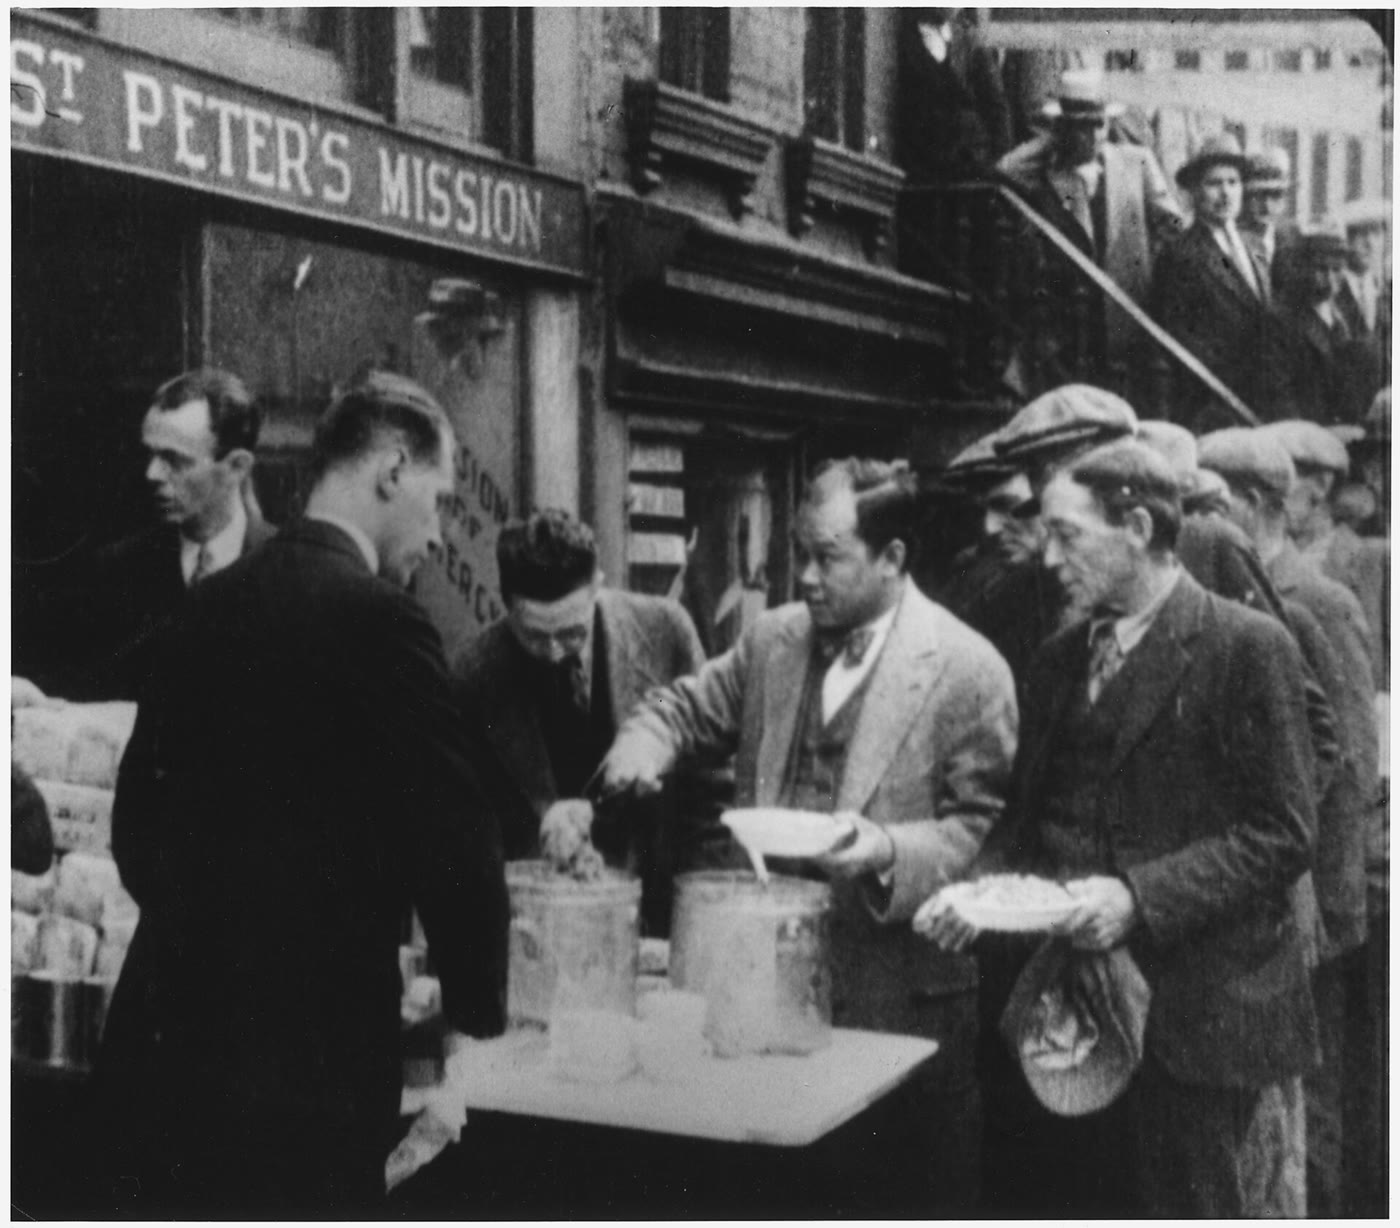
\includegraphics[width=0.58\linewidth]{images/book2/photos/g11-unemployment-breadline-1932.jpg}

{\small A breadline at a mission in New York City, about 1932: free food, paid for by private funds, for people out of work.}
\end{omfigure}

\section{Why wages do not clear the market}\label{sec:g11:unemployment:wages}

If wages fell whenever people were looking for work, \omterm{def:g11:unemployment:frictional}{structural unemployment} from wages would vanish. Three reasons they do not: contracts fix wages for a time; \omterm{def:g11:labour-market:minimum-wage}{minimum
wages} set a floor; and employers may choose to pay more than they must.

\begin{definition}[Efficiency wage]\label{def:g11:unemployment:efficiency-wage}
An \emph{efficiency wage}\index{efficiency wage} is a wage set above the level needed to attract workers, because it raises their effort, lowers quitting, or attracts
better applicants, so that it raises output by more than it costs.
\end{definition}

\begin{model}{Efficiency wages}
\assumes Employers cannot fully observe effort; a worker who loses a well-paid job loses more than one who loses a job paying the going rate.
\predicts Employers pay above the market-clearing wage; more people want such jobs than there are jobs; unemployment persists even with flexible wages.
\tested Consistent with the Ford Motor Company's five-dollar day of 1914 (record below), where queues formed and productivity rose; one
  firm's episode is not a test, which would compare many firms' pay, effort and queues.
\breaks Where effort is easy to observe and pay by the piece is possible.
\end{model}

\begin{record}[The five-dollar day, 1914]
% ledger: g11:rs1987
In 1914 the Ford Motor Company introduced a pay of five dollars a day for its car workers. A study of the episode (Raff and Summers 1987) concluded that the decision is best explained by labour
problems at the plants, that the new wage brought long queues of people seeking jobs at the company, and that significant rises in productivity and profits followed: a case in
which paying more than the market required paid for itself.
\end{record}

\section{Benefits, rules and policies}\label{sec:g11:unemployment:policies}

\begin{definition}[Replacement rate and employment protection]\label{def:g11:unemployment:replacement-rate}
The \emph{replacement rate}\index{replacement rate} is unemployment benefit as a share of the wage earned before. \emph{Employment protection}\index{employment
protection}\phantomsection\label{def:g11:unemployment:employment-protection} is the set of rules that make dismissing a worker costly or slow: notice, severance pay,
procedures.
\end{definition}

Benefits support people while they look for work, and they can let them look for a better match. In the flow model they can also lower the \omterm{def:g11:unemployment:separation-rate}{job-finding rate}, because a
job pays less over what one would receive without it. \omterm{def:g11:unemployment:replacement-rate}{Employment protection} lowers separations, but also hiring, since a worker hired is harder to let go; its effect on
the steady-state rate depends on which falls more. Training, wage subsidies and support for demand in recessions are the other main policies; each has to be judged by
studies of its effects, which differ widely by programme.

\begin{record}[Unemployment benefit duration and spell length]
% ledger: g11:ccw2007
Austrian rules give natural experiments: a severance payment of two months' pay, and unemployment benefits that last 30 weeks instead of 20, go to some workers and not to
others who are almost the same. Comparing such workers, a study found that the severance payment
lowered the \omterm{def:g11:unemployment:separation-rate}{job-finding rate} by 8 to 12\,\%, and the longer benefits lowered it by 5 to 9\,\% in the first 20 weeks of search, while the jobs eventually found were no
better.
\end{record}

\section{Exercises}

\begin{exercise}[$\star$]\label{exo:g11:unemployment:1}
Employed, unemployed or inactive? A full-time student not looking for work; a woman who lost her job, applied to three firms last week and can start on Monday; a man who
worked two hours for pay last week; a man who wants a job but stopped looking because he thinks there are none.
\end{exercise}

\begin{exercise}[$\star$]\label{exo:g11:unemployment:2}
Employed, unemployed or inactive? A person who has found a job that starts in two months and is available now; a retired person; a part-time worker who wants more hours;
a person who is looking for work but cannot start for six weeks.
\end{exercise}

\begin{exercise}[$\star$]\label{exo:g11:unemployment:3}
In a population aged 15 to 74 of 1000 people, 600 are employed, 40 unemployed and 360 inactive. Compute the labour force, the unemployment rate and the \omterm{def:g11:unemployment:employment-rate}{employment rate}.
\end{exercise}

\begin{exercise}[$\star$]\label{exo:g11:unemployment:4}
A labour force of 2000 has an unemployment rate of 8\,\%. How many are unemployed and employed? If the working-age population is 3000, what is the \omterm{def:g11:unemployment:employment-rate}{employment rate}?
\end{exercise}

\begin{exercise}[$\star$]\label{exo:g11:unemployment:5}
From the opening chart, which country has the highest youth unemployment rate and which the lowest? Compute the ratio of the youth rate to the total rate in Germany and in
Sweden.
\end{exercise}

\begin{exercise}[$\star\star$]\label{exo:g11:unemployment:6}
Monthly $s = 0.02$ and $f = 0.30$. Find the steady-state unemployment rate.
\end{exercise}

\begin{exercise}[$\star\star$]\label{exo:g11:unemployment:7}
Monthly $s = 0.015$ and $f = 0.135$. Find the steady state, and the share of the gap closed in one month.
\end{exercise}

\begin{exercise}[$\star\star$]\label{exo:g11:unemployment:8}
With yearly rates $s = 0.1$ and $f = 0.6$, unemployment starts at 20\,\%. Compute it after one, two and three years, and give its limit.
\end{exercise}

\begin{exercise}[$\star\star$]\label{exo:g11:unemployment:9}
In \cref{exo:g11:unemployment:6}, the \omterm{def:g11:unemployment:separation-rate}{job-finding rate} falls to 0.20. Find the new steady state.
\end{exercise}

\begin{exercise}[$\star\star$]\label{exo:g11:unemployment:10}
From the chart of 1870--2020, give the highest unemployment rate of each country in the 1930s, and the rates of the United States and Britain in 1982.
\end{exercise}

\begin{exercise}[$\star\star$]\label{exo:g11:unemployment:11}
Of 200 unemployed people, 70 have been out of work for a year or more. What is the long-term share? If every unemployed person finds a job with probability 0.1 each month,
what share of a group that becomes unemployed together is still unemployed a year later?
\end{exercise}

\begin{exercise}[$\star\star\star$]\label{exo:g11:unemployment:12}
What evidence would contradict the idea of a constant natural rate? Use the British figures from the chart of 1870--2020, and say what could make a natural rate move.
\end{exercise}

\begin{exercise}[$\star\star\star$]\label{exo:g11:unemployment:13}
A worker gains effort worth 30 dalens a month by shirking. Shirking is caught with probability 0.2 a month, and a worker caught loses his job and is paid 1500 dalens a month
for the next 10 months instead of his wage $w$. Above what wage does he not shirk?
\end{exercise}

\begin{exercise}[$\star\star\star$]\label{exo:g11:unemployment:14}
Monthly $s = 0.02$ and $f = 0.18$. Longer benefits lower the \omterm{def:g11:unemployment:separation-rate}{job-finding rate} by 7\,\%, the middle of the Austrian estimate. Find the steady state before and after.
\end{exercise}

\begin{exercise}[$\star\star\star$]\label{exo:g11:unemployment:15}
Give three reasons why the youth unemployment rate is higher than the total rate, and say which flow rate each acts on. Why might it be much lower in Germany and the
Netherlands than in Spain or Sweden?
\end{exercise}

\section{Problem: Brenland's Labour Flows}

\begin{problem}[{Weekend problem --- steady states, a recession and the way back}]
\label{pb:g11:unemployment:1}
Brenland's labour force has two groups. Group A, with upper secondary schooling, is 75\,\% of it, with monthly rates $s = 0.01$ and $f = 0.24$. Group B, without, is 25\,\%,
with $s = 0.02$ and $f = 0.18$. Each group's rate follows $u_{t+1} = s + (1 - s - f)u_t$.

\medskip
\noindent\textbf{Part I --- Steady states.}
\begin{enumerate}
\item Find the steady-state unemployment rate of each group.
\item Find Brenland's overall steady-state rate.
\item What share of the unemployed belong to group B?
\item What is the expected length of a spell of unemployment in each group, in months, if a spell ends with probability $f$ each month?
\item Which difference between the groups matters more for their steady states, $s$ or $f$?
\end{enumerate}

\medskip
\noindent\textbf{Part II --- A recession.}
\begin{enumerate}[resume]
\item For twelve months, $f$ falls to 0.15 in group A and to 0.10 in group B. Find the steady state each group would reach if this lasted.
\item Compute group A's rate after one month and after twelve.
\item Group B's rate after twelve months is 15.23\,\%. Check it with the formula of the proposition.
\item Compute Brenland's rate after twelve months.
\item By how many points has the gap between the groups widened?
\end{enumerate}

\medskip
\noindent\textbf{Part III --- The way back.}
\begin{enumerate}[resume]
\item After twelve months $f$ returns to normal. By what factor does each group's gap to its steady state shrink each month?
\item Find the number of months it takes each group to close half its gap.
\item Compute group A's rate three months after the recovery begins.
\item Why does group B take longer to recover?
\item The chart of Brenland's path in this chapter traces it. How far is Brenland from its steady state two years after the recession ends?
\end{enumerate}

\medskip
\noindent\textbf{Part IV --- Interpretation.}
\begin{enumerate}[resume]
\item Which part of Brenland's unemployment in month 12 is cyclical?
\item A training programme moves 10\,\% of the labour force from group B to group A. Find the new overall steady state.
\item Longer benefits lower group B's normal \omterm{def:g11:unemployment:separation-rate}{job-finding rate} to 0.16. Find its new steady state.
\item Why might the model understate how long recovery takes?
\item State the result of the problem: the steady-state unemployment rate of each group and of Brenland, and the months to close half the gap after the recession.
\end{enumerate}
\end{problem}
